\section{X-Project Architecture}
\label{sec:XPR_arc}

A Web application developed using the x-project toolkit, an x-project app, is a full stack JavaScript Single Page Application.

\subsection{Server Side}
\label{subsec:XPR_arc_serv}

On the server side, an X-Project app is based on NodeJS (see \ref{sec:TCH_nodejs}) used to create the server environment, MongoDB (see \ref{sec:TCH_mongodb}) used to storage data, and the Web framework Loopback by Strongloop (see \ref{sec:TCH_loopback}).

Node.js® is a JavaScript runtime built on Chrome's V8 JavaScript engine. Node.js uses an event-driven, non-blocking I/O model that makes it lightweight and efficient. Node.js' package ecosystem, npm, is the largest ecosystem of open source libraries in the world. L'utilizzo di NodeJS permette di creare un'applicazione verticale full-stack.

LoopBack generates model API from the models schemas, to let CRUD operations on models. Questo framework è al centro dell'architettura lato server del nostro progetto. Questo servizio ci permette di creare API in modo veloce e solo tramite la definizione di modelli.
LoopBack offre nel suo interno diversi connettori a database tra cui quello per MongoDB. 

MongoDB is a cross-platform document-oriented database. Classified as a NoSQL database, MongoDB eschews the traditional table-based relational database structure in favor of JSON-like documents with dynamic schemas. MongoDB è un database orientato al documento, non un DB relaionale e questo consente una facilità nella scalabilità orizzontale che il modello relazionale non possiede oltre ad altri numerosi benefici. Il concetto di righa è rimpiazzato da quello di documento, un modello più flessibile che permette di incorporare altri documenti ed array. Infatti con questo approccio document-oriented è possibile rappresentare delle relazioni gerarchiche anche molto complesse in un singolo record, comportandosi concettualmente in maniera molto simile ad un linguaggio di programmazione Object-Oriented.


\subsection{Client Side}
\label{subsec:XPR_arc_clie}

On the client side, an X-Project app is based on HTML5 Web Components via Polymer-Project by Google.
On the top of this stack lies X-Elements a se of Polymer elements for local routing, API request, forms, lists, style and admin pages, as listed further (see \ref{sec:XPR_xel}).


\begin {figure}[h]
\graphicspath{{images/chapter_xpr/}}
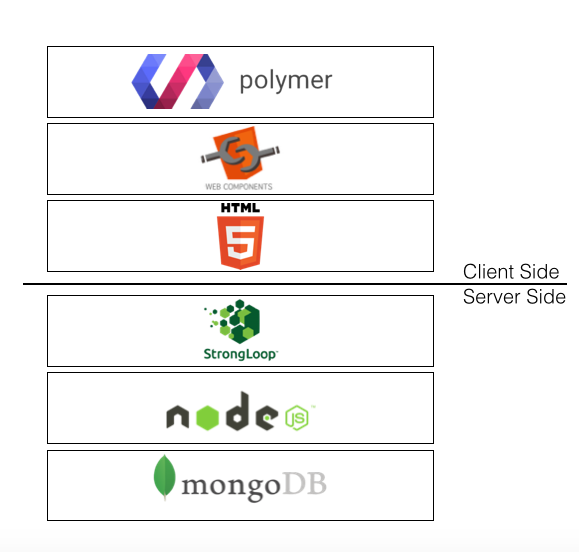
\includegraphics[width=\textwidth]{XPR_stack}
\caption{X-Project Architectural Stack }
\end {figure}